% Correcting the title chapter page
\fancypagestyle{plain}{%
    \fancyhf{}
    \fancyhead[RO,LE]{\bfseries \thepage}
    \fancyhead[CO]{\rightmark}
    \fancyhead[CE]{\leftmark}
    \renewcommand{\headrulewidth}{0.4pt}}


\chapter{Svojstva ireducibilnih reprezentacija}

\section{Schurove leme}

Sva ključna svojstva ireducibilnih reprezentacija slijede iz 
dvije Schurove leme.

\begin{teorem}[Prva Schurova lema]
Neka operator S povezuje dvije  ireducibilne
reprezentacije $\Gamma=\{D(g)\}$ i $\Gamma'=\{D'(g)\}$ u smislu da je
\begin{displaymath}
  SD(g)=D'(g)S  \quad \forall g\in G  \;.
\end{displaymath}
Tada je ili $S=0$ ili je $S$ invertibilan i imamo
\begin{displaymath}
D(g)=S^{-1}D'(g)S
\end{displaymath}
tj. dvije su reprezentacije ekvivalentne. (Mogućnost
da je $S$ singularan, ali ne i nul-operator je isključena.)
\end{teorem}

\centerline{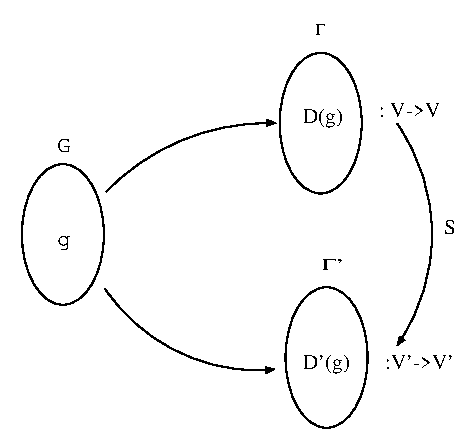
\includegraphics[scale=0.8]{pics/schur.eps}}

\emph{Dokaz.}
Neka su $V$ i $V'$ vektorski prostori na kojima djeluju $\Gamma$ i $\Gamma'$.
Slika $S(V)$ prostora $V$, $S(V)=\{S\vec{x} \td x \in V \}$, je potprostor od $V'$. 
Sva potrebna svojstva
$S(V)$ nasljeđuje od $V'$, a zatvorenost i egzistencija inverza su 
posljedice linearnosti operatora $S$.
Dodatno, $S(V)$ je \emph{invarijantni} potprostor od $V'$ jer
$$D'(g)S\vec{x}=SD(g)\vec{x} \in S(V)\,.$$

Kako je $\{D'(g)\}$ ireducibilna, iz
definicije ireducibilnosti \ref{def:irrep} slijedi
da je ili $S(V)=\{\vec{0'}\}$ ili $S(V)=V'$.

\begin{enumerate}
\item Ako je $S(V)=\{\vec{0'}\}$ tj. svi vektori domene operatora $S$
    preslikavaju se u nul-vektor, to znači da je $S$ nul-operator,  $S=0$.
    To je prva od dvije mogućnosti iz prve Schurove leme.

\item Neka je $S(V)=V'$ tj. $S$ je surjekcija. Promotrimo 
    kernel Ker($S$) koji je zahvaljujući linearnosti od $S$
    potprostor od $V$.
    Uzmimo proizvoljni vektor $\vec{k}$ iz Ker($S$).
    Po pretpostavci leme je 
    $$ S D(g) \vec{k} = D'(g)S\vec{k} = \vec{0'}$$
    što znači da je i $D\vec{k}$ element kernela Ker($S$), odnosno
    i kernel je \emph{invarijantni} potprostor, baš kao i slika.
    Sad, kako je $\{D(g)\}$ ireducibilna slijedi da je ili
    Ker($S$)=$\{\vec{0}\}$ ili Ker($S$)=$V$.
    Ker($S$)$=V$ ne može biti jer onda ne bi bilo $S(V)=V'$ nego bi bilo
      $S(V)=\vec{0'}$.
    Zaključujemo da je Ker($S$)$=\{\vec{0}\}$ pa je $S$ i injekcija (cf.
    teorem \ref{th:izomorfizam} o izomorfizmu) te ima inverz
    i onda iz pretpostavke leme slijedi $D(g)=S^{-1}D'(g)S$, tj.
    dvije su reprezentacije ekvivalentne, što je druga mogućnost leme.\qed 
\end{enumerate}

\begin{teorem}[Druga Schurova lema]
Operator koji komutira sa svim operatorima neke ireducibilne 
reprezentacije
\begin{displaymath}
  D(g)S=SD(g) \quad \forall g\in G
\end{displaymath}
je nužno proporcionalan jediničnom operatoru
(identiteti), $S = \lambda \Eins$.
\end{teorem}

\emph{Dokaz.} Iz fundamentalnog teorema algebre slijedi da $S$ ima
barem jedan svojstveni vektor tj. da postoji
$\vec{x}\neq\vec{0}$ takav da je $S\vec{x}=\lambda\vec{x}$.
To možemo zapisati i u obliku $(S-\lambda\Eins)\vec{x}=0$ što
znači da je $(S-\lambda\Eins)$
singularna matrica (neki vektor $\neq \vec{0}$ preslikava u
$\vec{0'}$ pa nije injekcija).
No, $[S-\lambda\Eins, D(g)]=0$
jer jedinični operator komutira trivijalno, a $S$ komutira po pretpostavci leme.
No onda je po prvoj Schurovoj lemi $S-\lambda\Eins$ nul-operator jer smo upravo vidjeli
da nije regularan. Iz $S-\lambda\Eins=0$ onda odmah slijedi $S=\lambda\Eins$.\qed



\section{Relacije ortogonalnosti i karakteri}
\label{sec:ortogonalnost}

Promotrimo dvije ireducibilne reprezentacije, $\Gamma_{\alpha}$ i $\Gamma_{\beta}$,
koje djeluju na vektorskim prostorima $V^{(\alpha)}$ i $V^{(\beta)}$,
dimenzija $d_\alpha$ i $d_\beta$.
Ako je $\alpha\neq\beta$ podrazumijevat ćemo da su reprezentacije neekvivalentne.
Promotrimo i proizvoljni operator $A$ koji preslikava s $V^{(\beta)}$ na  $V^{(\alpha)}$.
Dakle imamo
\begin{align*}
D^{(\alpha)} &: V^{(\alpha)} \to V^{(\alpha)}\,, \\
D^{(\beta)}  &: V^{(\beta)}  \to V^{(\beta)} \,, \\
A          &: V^{(\beta)} \to V^{(\alpha)} \,.
\end{align*}
Definirajmo sada matricu
\begin{equation*}
B\equiv \sum_{g\in G} D^{(\alpha)}(g) A D^{(\beta)}(g^{-1}) \;.
\end{equation*}
Pokazat ćemo da $B$ zadovoljava pretpostavke Schurovih lema.
Uzimimo proizvoljni element $h\in G$. Tada vrijedi:
\begin{equation*}
\begin{split}
 D^{(\alpha)}(h)B &= \sum_g D^{(\alpha)}(h) D^{(\alpha)}(g) A
    D^{(\beta)}(g^{-1}) \\
&= \sum_g D^{(\alpha)}(hg) A D^{(\beta)}(g^{-1}) \\
&= ( \textrm{zamjenom}\; hg\equiv g' \, , \; g^{-1}=g'^{-1}h ) \\
&= \sum_{g'} D^{(\alpha)}(g') A D^{(\beta)}(g'^{-1}h) \\
&= \sum_{g'} D^{(\alpha)}(g') A D^{(\beta)}(g'^{-1}) D^{(\beta)}(h) \\
&= B D^{(\beta)}(h)
\end{split}
\end{equation*}

U slučaju $\alpha\neq\beta$ ($\Gamma_\alpha$ i $\Gamma_\beta$ nisu 
ekvivalentne),
iz prve Schurove leme slijedi da je $B=0$. Ako je pak $\alpha=\beta$, tj.
$D^{(\alpha)}(h)=D^{(\beta)}(h)$ onda iz druge Schurove leme
slijedi $B=\lambda \Eins$.
Ove se dvije tvrdnje mogu kompaktno ujediniti u relaciju
\begin{equation}
  B = \sum_g D^{(\alpha)}(g) A D^{(\beta)}(g^{-1}) =
 \lambda^{(\alpha)}_A \delta^{\alpha\beta} \Eins \;,
\end{equation}
odnosno, po komponentama,
\begin{equation}
\sum_g D^{(\alpha)}_{ir}(g) A_{rs} D^{(\beta)}_{sl}(g^{-1})
 = \lambda_{A}^{(\alpha)} \delta^{\alpha\beta} \Eins_{il} \,.
 \label{eq:ortpokomp}
\end{equation}
$A$ je ovdje bila proizvoljna matrica. Uzmimo sada konkretnije na mjesto $A$
matricu $A^{(j,k)}$ koja je svugdje nula osim što joj je
element $A^{(j,k)}_{jk}=1$
\begin{displaymath}
 A^{(j,k)}=
\begin{array}{cc}
 & \cdots k \cdots \\
        \begin{array}{c}
         \cdot \\ \cdot \\ j \\ \cdot \\ \cdot \\ \cdot 
        \end{array}
 & 
\begin{pmatrix}
  & \cdot & \\
  & \cdot & \\
 \cdots & 1  & \cdots \\
  & \cdot & \\
  & \cdot & \\
  & \cdot & \\
\end{pmatrix} \,,
\end{array}
\end{displaymath}
\begin{displaymath}
A^{(j,k)}_{rs}=\delta_{rj}\delta_{sk} \,.
\end{displaymath}

Upotrebom te matrice u gornjoj relaciji (\ref{eq:ortpokomp})  dobivamo
\begin{equation}
\sum_g D^{(\alpha)}_{ij}(g) D^{(\beta)}_{kl}(g^{-1}) = 
 \lambda^{(\alpha)}_{jk} \delta^{\alpha\beta} \Eins_{il} \;.
\end{equation}
Sada treba odrediti $\lambda_{jk}$. 
Stavimo ovdje $\alpha =\beta$ i uzmimo trag po $il$ indeksima
množenjem s $\delta_{il}$,
\begin{displaymath}
\sum_g D^{(\alpha)}_{ij}(g) D^{(\alpha)}_{ki}(g^{-1}) = 
 \lambda^{(\alpha)}_{jk} \delta^{\alpha\alpha}\, \textrm{dim}(V^{(\alpha)})
 \equiv \lambda^{(\alpha)}_{jk} d_{\alpha} \,.
\end{displaymath}
S druge strane, to je također jednako
\begin{displaymath}
 \sum_g D(g^{-1}g)_{kj}=\sum_g D(e)_{kj}= \sum_g \Eins_{kj} = \delta_{kj} \sum_g 
 = \delta_{kj} n \;.
\end{displaymath}
Ovdje je $n$ red grupe G.
Slijedi da je
\begin{displaymath}
\lambda^{(\alpha)}_{jk}= \frac{n}{d_{\alpha}}\delta_{kj} \;,
\end{displaymath}
što daje \emph{temeljni teorem o ortogonalnosti} matrica ireducibilnih
reprezentacija:
\begin{teorem}[Ortogonalnost matrica ireducibilnih reprezentacija]
\begin{displaymath}
\sum_g D^{(\alpha)}_{ij}(g) D^{(\beta)}_{kl}(g^{-1}) =
 \frac{n}{d_{\alpha}}\delta^{\alpha\beta}\delta_{il}\delta_{kj} \;.
\end{displaymath}
\label{tm:ortogonalnost}
\end{teorem}

Nadalje, uvijek možemo uzeti da je $D^{(\beta)}(g)$ unitarna matrica
i u tom slučaju je
\begin{displaymath}
\sum_g D^{(\alpha)}_{ij}(g) D^{(\beta)}_{lk}(g)^* =
 \frac{n}{d_{\alpha}}\delta^{\alpha\beta}\delta_{il}\delta_{kj} \;.
\end{displaymath}
Stavimo ovdje $\alpha=\beta$ i promotrimo skup od $d^{2}_\alpha$ vektora
$\vec{x}_{ij}$ iz novog $n$-dimenzionalnog vektorskog prostora,  čije
su komponente dane komponentama svih matrica reprezentacije:
\begin{displaymath}
\vec{x}_{ij} \equiv
(D^{(\alpha)}_{ij}(g_1), D^{(\alpha)}_{ij}(g_2), \ldots, 
D^{(\alpha)}_{ij}(g_n)) \,.
\end{displaymath}
(Ne miješati ovaj
prostor s $V^{\alpha}$ koji je dimenzije $d_\alpha$!) Zbog
\begin{displaymath}
\sum_g D^{(\alpha)}_{ij}(g) D^{(\alpha)}_{lk}(g)^* = (\vec{x}_{lk},\vec{x}_{ij})
 =\frac{n}{d_{\alpha}}\delta_{il}\delta_{kj}
\end{displaymath}
vektori $\vec{x}_{ij}$ su međusobno ortogonalni.
Za neku drugu ireducibilnu reprezentaciju 
$\Gamma_{(\alpha')}$ imamo novih $d_{\alpha'}^{2}$
vektora  koji su ortogonalni međusobno, ali i obzirom na prvih
$d_{\alpha}^{2}$ vektora. Treća ireducibilna reprezentacija daje novih $d_{\alpha''}^{2}$ itd.
No znamo da je općenito maksimalan broj ortogonalnih 
vektora u $n$-dimenzionalnom vektorskom prostoru upravo $n$.
Tako slijedi
\begin{equation}
\sum_{\alpha} d_{\alpha}^{2} \leq n   \,,
\label{eq:sumdlen}
\end{equation}
pa kako je svaka ireducibilna reprezentacija barem jednodimenzionalna
i\-ma\-mo $\sum_{\alpha} d_\alpha \leq n$ tj.
broj ireducibilnih reprezentacija je manji ili jednak broju elemenata grupe.
Štoviše, vrijedi (vidi npr. \cite{Hamermesh:1989}) da je nejednakost
(\ref{eq:sumdlen}) saturirana tj.
\begin{displaymath}
\sum_{\alpha} d_{\alpha}^2 = n \;.
\end{displaymath}
Da bismo odredili broj članova u ovoj relaciji tj.
broj (neekvivalentnih) ireducibilnih reprezentacija grupe, treba nam
pojam \emph{karaktera} reprezentacije.
\begin{definicija}[Karakter reprezentacije]
Karakter $\chi$ reprezentacije $\Gamma=\{D(g)\}$ grupe $G$ je skup
$\chi=\{\chi(g) = \Tr D(g) \td  g\in G\}$.
\end{definicija}
Prvo važno svojstvo je da ekvivalentne reprezentacije imaju iste
karaktere jer zbog cikličnosti traga
imamo $\Tr S D(g) S^{-1} = \Tr D(g)$.
Bez dokaza navedimo da vrijedi i obrat: jednakost karaktera implicira
da su reprezentacije ekvivalentne.
(Usput, taj obrat se \emph{ne} poopćuje na beskonačne kontinuirane grupe, osim
  ukoliko nisu kompaktne, vidi \cite[302]{Cornwell:1997})
Zahvaljujući cikličnosti traga vidimo i da je
$\chi(g)=\Tr D(g) = \Tr D(h) D(g) D^{-1}(h) = \Tr D(hgh^{-1})$
  tj. konjugirani elementi imaju iste karaktere (Oprez: Treba
  razlikovati karakter reprezentacije $\chi$ od njegove komponente
  $\chi(g)$ koju isto često zovemo karakter --- karakter elementa.)

Za unitarnu reprezentaciju vrijedi $\chi(g^{-1}) = \Tr D(g^{-1})= \Tr D^{\dagger}
    = \chi^{*}(g)$.


Uzmimo sada trag po obje matrice
u teoremu o ortogonalnosti \ref{tm:ortogonalnost} množenjem
s $\delta_{ij}\delta_{kl}$ pa dobijemo
\begin{displaymath}
\sum_g \chi^{(\alpha)}(g) \chi^{(\beta)}(g)^* = 
\frac{n}{d_{\alpha}} \delta^{\alpha\beta} \delta_{ik}\delta_{ki} =
\frac{n}{d_{\alpha}} \delta^{\alpha\beta} d_{\alpha} =
n \delta^{\alpha\beta} \;.
\end{displaymath}

Definiramo li skalarni produkt karaktera na sljedeći način
 \begin{displaymath}
(\chi, \phi) \equiv \frac{1}{n} \sum_g \chi(g) \phi(g)^* = (\phi, \chi) \;,
\end{displaymath}
imamo
\begin{displaymath}
(\chi^{(\alpha)}, \chi^{(\beta)}) = \delta^{\alpha\beta}
\end{displaymath}
tj. karakteri neekvivalentnih ireducibilnih reprezentacija su ortonormirani
obzirom na taj skalarni produkt.

Neka je sada $k_i$ broj elemenata u $i$-toj klasi konjugacije grupe $G$.
Tada, budući da su karakteri svih elemenata jedne klase konjugacije
isti imamo
\begin{displaymath}
(\chi^{(\alpha)}, \chi^{(\beta)})=\frac{1}{n} \sum_{i=1}^{k}  k_i
 \chi^{(\alpha)}_i \chi^{(\beta)*}_{i} = \delta^{\alpha\beta} \;.
\end{displaymath}
što je iskaz ortogonalnosti vektora u $k$-dimenzionalnom vektorskom
prostoru, gdje je $k$ broj klasa konjugacije grupe. Ortogonalni vektori su
\begin{displaymath}
\vec{\chi}^{(\alpha)} = (\chi^{(\alpha)}_1, \chi^{(\alpha)}_2, \ldots,
 \chi^{(\alpha)}_{k}) \,.
\end{displaymath}
Svaka ireducibilna reprezentacija daje jedan takav $k$-dimenzionalni vektor.
Istim logičkim slijedom kao i ranije ova ortogonalnost vodi na zaključak 
da je broj
ireducibilnih reprezentacija  manji ili jednak broju klasa konjugacije. Štoviše, vrijedi
(vidi literaturu) ortogonalnost vektora:
\begin{displaymath}
\vec{\chi}_i = (\chi^{(\alpha)}_i, \chi^{(\beta)}_i, \ldots)
\end{displaymath}
tj.
\begin{displaymath}
\frac{1}{n} \sum_{\alpha} k_i \chi^{(\alpha)}_i \chi^{(\alpha)*}_j =
\delta_{ij} \,,
\end{displaymath}
što na isti način daje suprotnu nejednakost da je broj klasa konjugacije manji
ili jednak broju ireducibilnih reprezentacija.
Zaključujemo da je broj ireducibilnih reprezentacija grupe 
upravo jednak broju njenih klasa konjugacije!

\section{Tablice karaktera}

\emph{Tablica karaktera} neke grupe je tablica karaktera svih njenih
ireducibilnih reprezentacija.
\begin{center}
    \setlength{\tabcolsep}{12pt}
    \renewcommand{\arraystretch}{2.0}
\begin{tabular}{c|cccccc}
               & \multicolumn{6}{c}{Klase konjugacije} \\ \hline
  $\Gamma_{\alpha}$ & $\chi_{1}^{(\alpha)}$ & $\chi_{2}^{(\alpha)}$ & $\cdot$ &
       $\cdot$ & $\cdot$ & $\chi_{k}^{(\alpha)}$ \\
  $\Gamma_{\beta}$  & $\chi_{1}^{(\beta)}$  & $\cdot$ & $\cdot$ & $\cdot$ & $\cdot$  & $\cdot$ \\
     $\cdot$ &  $\cdot$   & $\cdot$ & $\cdot$ & $\cdot$ & $\cdot$  & $\cdot$ \\
     $\cdot$ &  $\cdot$   & $\cdot$ & $\cdot$ & $\cdot$ & $\cdot$  & $\cdot$ \\
\end{tabular}
    \renewcommand{\arraystretch}{1.0}
\end{center}
Vidjet ćemo da tablica često daje dovoljno informacija za praktične primjene, a može
se, pomoću slijedećih pravila, konstruirati i bez eksplicitnog
poznavanja samih matrica reprezentacija i uzimanja njihovih tragova.

\subsection*{Pravila za konstrukciju tablice karaktera}

\begin{enumerate}

\item Broj ireducibilnih reprezentacija jednak je broju klasa konjugacije 
  grupe. Iz ovoga slijedi da tablica ima jednak broj redova i stupaca. 
  Broj klasa pronalazimo "pješke," analizom grupe.

\item Kako su dimenzije vektorskih prostora prirodni brojevi,
    uvjet da je zbroj kvadrata dimenzija ireducibilnih reprezentacija
    jednak broju elemenata grupe, $\sum_{\alpha} d_{\alpha}^2 = n$, često ima jedinstveno rješenje koje
    određuje dimenzionalnosti $d_{\alpha}$ svih ireducibilnih reprezentacija.

\item Jedinični element grupe je klasa za sebe, a reprezentiran je uvijek
  jediničnom matricom $D^{(\alpha)}(e)=\Eins$ čiji je 
   karakter $\chi^{(\alpha)}(e)=d_{\alpha}$.
  Ovo određuje jedan (konvencionalno prvi) stupac tablice.

\item Uvijek postoji trivijalna jednodimenzionalna ireducibilna
   reprezentacija  $D(g)=\chi(g)=1$, $\forall g\in G$.
  Dakle jedan red (konvencionalno prvi) se sastoji od samih jedinica.

\item Za jednodimenzionalne reprezentacije vrijedi $D(g)=\chi(g)$ pa
  sami karakteri reprezentiraju grupu i njihovo množenje mora biti
  homomorfno množenju odgovarajućih elemenata grupe.

\item  \[\sum_{i=1}^{k} k_{i} \chi^{(\alpha)}_{i} \chi^{(\beta) *}_{i} =
    n \delta^{\alpha\beta}\] 
(\emph{Redovi} tablice su ortogonalni i, kad se uzmu u obzir težinski
  faktori $k_i$, normirani su na $n$)

\item  \[\sum_{\alpha=1}^{k} k_{i} \chi^{(\alpha)}_{i} \chi^{(\alpha) *}_{j} =
    n \delta_{ij} \] 
(\emph{Stupci} tablice su ortogonalni i, kad se uzmu u obzir težinski
  faktori $k_i$, normirani su na $n$)

\end{enumerate}

Pravila je najbolje primjenjivati po redu jer su ona s većim rednim
brojem teža za primjenu i rjeđe nužna za kompletiranje tablice.

\begin{primjer}[Tablica karaktera grupe $\mathrm{D}_3$]
    \label{pr:karakteriD3}
Grupa ima tri klase konjugacije (vidi primjer \ref{pr:klaseD3}):

\begin{center}
\begin{enumerate}[label=$K_{\mathrm{\arabic{enumi}}}$]
 \item $ = \{e\}$
 \item $ = \{c, c^2\}$
 \item $ =  \{ b, bc, bc^2 \}$
\end{enumerate}
\end{center}

Iz pravila 1) onda znamo da D$_{3}$ ima tri ireducibilne reprezentacije
i tablica karaktera će biti $3 \times 3$
\begin{center}
\begin{tabular}{c|ccc}
  & $K_1$ & $2 K_2$  & $ 3 K_3$ \\ \hline
$\Gamma_1$ &   &  &   \\
$\Gamma_2$ &   &  &   \\
 $\Gamma_3$  &   &  &  
\end{tabular}
\end{center}
Ovdje smo prema običaju uz naziv klase stavili i broj njenih elemenata. To je
korisno imati pri ruci jer su to težinski faktori potrebni za primjenu
pravila 6) i 7).
Pravilo 2) vodi na jednadžbu
 $$\sum_{\alpha=1}^{3} d_{\alpha}^2 = d_{1}^2 + d_{2}^2
   + d_{3}^2 = n = 6 $$
koja, do na permutacije, ima samo jedno rješenje u skupu prirodnih brojeva
 $$ d_1 = d_2 = 1\,,\quad d_3=2 \,. $$
Dakle, dvije su reprezentacije jednodimenzionalne. Običaj je organizirati
tablicu tako da dimenzionalnost raste idući dolje po retcima.
Po pravilu 3) prvi stupac su karakteri jediničnih matrica tj. dimenzionalnosti
reprezentacija
\begin{center}
\begin{tabular}{c|ccc}
  & $K_1$ & $2 K_2$  & $ 3 K_3$ \\ \hline
$\Gamma_1$ & 1 &  &   \\
$\Gamma_2$ & 1 &  &   \\
 $\Gamma_3$  & 2 &  &  
\end{tabular}
\end{center}
a po pravilu 4) prvi red pripada trivijalnoj reprezentaciji čiji su svi karakteri
jedinice:
\begin{center}
\begin{tabular}{c|ccc}
  & $K_1$ & $2 K_2$  & $ 3 K_3$ \\ \hline
$\Gamma_1$ & 1 & 1 & 1   \\
$\Gamma_2$ & 1 &  &   \\
 $\Gamma_3$  & 2 &  &  
\end{tabular}
\end{center}
Drugi redak možemo kompletirati korištenjem pravila 5) obzirom da je $\Gamma_2$
jednodimenzionalna. Uporaba pravila nije sasvim algoritamska, ali od koristi je promatrati
umnoške karaktera različitih klasa. Npr. $\chi^{(2)}(b)\chi^{(2)}(c)=\chi^{(2)}(bc)$
po svojstvu homomorfizma. Kako elementi $b$ i $bc$ pripadaju istoj klasi,
$\chi^{(2)}(b)=\chi^{(2)}(bc)$
i možemo ih skratiti s obje strane (ne mogu biti nula jer je npr. 
$\chi^{(2)}(b)^2 = \chi^{(2)}(b^2) =
\chi^{(2)}(e) = 1$) i slijedi da je $\chi^{(2)}(c)=1$. Upravo smo pokazali i da je 
  $\chi^{(2)}(b)^2=1$ tj. $\chi^{(2)}(b)=\pm 1$.
Sad se oslanjamo na pravilo 6) da bi zaključili da kad bi bilo 
$\chi^{(2)}(b)=1$ prva dva reda bi bila jednaka, a ne
ortogonalna. Tako znamo da je $ \chi^{(2)}(b)=-1$ i imamo
\begin{center}
\begin{tabular}{c|ccc}
  & $K_1$ & $2 K_2$  & $ 3 K_3$ \\ \hline
$\Gamma_1$ & 1 & 1 & 1   \\
$\Gamma_2$ & 1 & 1 & -1   \\
 $\Gamma_3$  & 2 & a  & b  
\end{tabular}
\end{center}
Ovdje smo s $a$ i $b$ označili zadnja dva nepoznata elementa tablice koje ćemo
odrediti pomoću pravila 6) tj. ortogonalnosti trećeg retka s prvim i drugim,
gdje treba paziti na težinske faktore. Imamo
\begin{align*}
    \sum_{i=1}^{3} k_{i} \chi^{(3)}_{i} \chi^{(1) *}_{i}& =
      2+2a+3b=0 \,, \\
    \sum_{i=1}^{3} k_{i} \chi^{(3)}_{i} \chi^{(2) *}_{i}& =
      2+2a-3b=0  \,,
\end{align*}
što su dvije jednadžbe s dvije nepoznanice i s rješenjem $a=-1, b=0$.
Tako smo odredili cijelu tablicu. Običaj je za označavanje ireducibilnih
reprezentacija i klasa konjugacija koristiti kristalografske
oznake. Mi ćemo koristiti tzv. Sch\"{o}nfliesove oznake iz priloga \ref{sec:kristalografija} 
pa konačna tablica izgleda ovako:
\begin{center}
\begin{tabular}{c|ccc}
  & E & 2$C_3$  & 3$C_2$ \\ \hline
$A_1$ & 1 & 1& 1 \\
$A_2$ & 1 & 1&-1 \\
 $E$  & 2 &-1& 0
\end{tabular}
\end{center}
Uvjerite se da je i pravilo 7), ortogonalnost stupaca tablice, zadovoljeno.
\end{primjer}

\begin{primjer}[Tablica karaktera grupe C$_3$]

Grupa C$_3$=$\{e, c, c^2\}$ je Abelova pa je svaki element klasa za sebe.
Dakle imamo tri klase i tri ireducibilne reprezentacije,
a iz pravila 2) slijedi $d_{1}^2+d_{2}^2+d_{3}^2 = n =3$
i vidimo da su sve tri jednodimenzionalne.
Pravila 3) i 4) nas vode na to da su prvi red i prvi stupac
tablice same jedinice.
Pravilo 5) se može upotrijebiti da se zaključi da
je$\chi(c)^3=\chi(c^3)=\chi(e)=1$ iz čega slijedi da su $\chi(c)$
kubni korijeni jedinice $\chi(c) = \exp(2\pi i k/3), k=0, 1, 2$,
odnosno mogućnosti su $\chi(c)=1, \omega\equiv e^{2\pi i/3}, \omega^2$.
Uvjeti ortogonalnosti redaka i stupaca nas onda vode na
strukturu:
\begin{center}
\begin{tabular}{c|ccc}
  & E & $c=C_3$  & $c^2=C_{3}^2$ \\ \hline
$\Gamma_{1}$ & 1 & 1& 1 \\
$\Gamma_{2}$  & 1 & $\omega$ &$\omega^2$  \\
$\Gamma_{3}$  & 1 &$\omega^2$ & $\omega$ 
\end{tabular}
\end{center}
Kako je $\omega^2 = \omega^* $ vidimo da
su $\Gamma_2$ i $\Gamma_3$ međusobno kompleksno
konjugirane reprezentacije (cf. zadatak \ref{zad:complex}).
Kompleksna konjugacija je sama po sebi isto svojevrsna transformacija
simetrije. Ukoliko proširimo razmatranje i na tu transformaciju $\Gamma_2$
i $\Gamma_3$ prestaju biti ireducibilne i zato se često te dvije reprezentacije
zajedno smatraju jednom dvodimenzionalnom ireducibilnom reprezentacijom $E$.
\end{primjer}


Zgodno je uočiti da neabelovska grupa $D_3$ ima i dvodimenzionalnu, dakle matričnu,
ireduciblinu reprezentaciju. To je logično jer neabelovsko svojstvo ne može biti
vjerno reprezentirano jednodimenzionalnim reperezentacijama.

\section{Dekompozicija reducibilnih reprezentacija}

Konstrukcijom tablice karaktera smo istovremeno i identificirali sve ireducibilne
reprezentacije grupe. Preostaje nam drugi zadatak obećan na kraju prošlog poglavlja,
a to je naučiti kako proizvoljnu reprezentaciju reducirati na direktan zbroj
ireducibilnih.  Uzmimo neku, moguće reducibilnu, reprezentaciju $\Gamma$. Općenito
\begin{displaymath}
  \Gamma = \Gamma_{1}\oplus\Gamma_{2}\oplus\cdots =
     \sum_{\alpha} \oplus a_{\alpha} \Gamma_{\alpha}
\end{displaymath}
gdje su $\Gamma_{\alpha}$ ireducibilne reprezentacije i
gdje je $a_{\alpha}$ \emph{multiplicitet} (broj pojavljivanja) 
$\Gamma_{\alpha}$ u $\Gamma$.
Uzmemo li sad trag nekog operatora iz $\Gamma$ iz  $i$-te klase konjugacije
imajući u vidu blok-dijagonalnu formu direktnog zbroja vidimo da je
\begin{equation}
  \chi_i = \sum_{\alpha}  a_{\alpha} \chi^{(\alpha)}_i \quad 
  \forall i  \,.
\end{equation}
Sada pomnožimo ovu realaciju s $k_i \chi^{(\beta)*}_i$, gdje je $\Gamma_{\beta}$
neka konkretna ireducibilna reprezentacija, te prosumiramo po svim klasama
i iskoristimo ortogonalnost karaktera ireducibilnih reprezentacija
\begin{equation}
\sum_{i=1}^{k} k_i \chi_i \chi^{(\beta)*}_i =
\sum_{\alpha}  a_{\alpha} \sum_{i=1}^{k} k_i\chi^{(\alpha)}_i \chi^{(\beta)*}_i
=\sum_{\alpha}  a_{\alpha} n \delta^{\alpha \beta} = n a_{\beta} \,.
\end{equation}
Tako dobivamo izraz za multiplicitet pojedine ireducibilne reprezentacije u
rastavu proizvoljne reprezentacije
\begin{equation}
a_{\alpha} = \frac{1}{n} \sum_{i=1}^{k}  k_i \chi_i \chi^{(\alpha)*}_i
\equiv (\chi^{(\alpha)}, \chi) \,,
\label{eq:multiplicitet}
\end{equation}
gdje smo uveli skalarni produkt karaktera $(\;,\;)$.

\begin{primjer}[Reprezentacija $\Gamma_V$ grupe D$_3$ na 3D euklidskom prostoru]
Promotrimo reprezentaciju grupe D$_3$ na standardnom trodimenzionalnom
vektorskom prostoru. (Oznaka $V$ implicira da mislimo na prave (polarne)
vektore, za razliku od "nepravih", aksijalnih ili pseudovektora koje obično
označavamo s $A$, vidi odjeljak \ref{sec:aksijalni}.) Kako nam trebaju samo
karakteri, dovoljno je promatrati po jednog reprezentanta svake od triju klasa
(vidi primjer \ref{pr:klaseD3}).
Jedinični element je naravno reprezentiran jediničnom matricom
$D^{(V)}(e)=\textrm{diag}(1,1,1)$ s karakterom 3.
Za reprezentanta klase $\{c, c^2\}$ možemo uzeti matricu rotacije
za 2$\pi$/3 oko $z$-osi
\begin{equation}
D^{(V)}(c)=
\begin{pmatrix}
-1/2 & -\sqrt{3}/2 & 0 \\
\sqrt{3}/2 & -1/2 & 0 \\
0 & 0 & 1
\end{pmatrix} \,.
\end{equation}
Za reprezentanta zadnje klase $\{b, bc, bc^2\}$ možemo uzeti matricu
rotacije za kut $\pi$ oko $y$-osi  koja naprosto izvrće $x$ i $z$
komponente vektora
\begin{equation}
D^{(V)}(b)=
\begin{pmatrix}
-1 & 0 & 0 \\
0 & 1 & 0 \\
0 & 0 & -1
\end{pmatrix} \,.
\label{eq:DVbD3}
\end{equation}
Uzimajući tragove, vidimo da je cijeli karakter ove reprezentacije
$\chi=(3,0,-1)$.
Kako smo u primjeru \ref{pr:karakteriD3} upoznali sve ireducibilne
reprezentacije, dvije jednodimenzionalne i jednu dodimenzionalnu,
znamo da je $\Gamma_V$ reducibilna. Njen rastav dobijemo izračunom 
multipliciteta svake pojedine od tri
ireducibilne reprezentacije pomoću skalarnog produkta (\ref{eq:multiplicitet}):
\begin{align*}
    a_{A_1}& = (\chi, \chi^{(A_1)})=\frac{1}{n}\sum_{i=1}^{3} k_i \chi_i \chi^{(A_1)*}_i \\
 & = \frac{1}{6}(1\cdot 3\cdot 1 + 2\cdot 0\cdot 1 + 3\cdot (-1) \cdot 1)=0\\
    a_{A_2}& = (\chi, \chi^{(A_2)}) \\
 & =\frac{1}{6}(1\cdot 3\cdot 1 + 2\cdot 0\cdot 1 + 3\cdot (-1)\cdot(-1))=1\\
    a_{E}& = (\chi, \chi^{(E)}) \\
 & =\frac{1}{6}(1\cdot 3\cdot 2 + 2\cdot 0\cdot (-1) + 3\cdot (-1)\cdot 0)=1
\end{align*}
Tako konačno imamo
\begin{equation}
\Gamma_V  = A_2 \oplus E \,.
\end{equation}
Od interesa je odrediti i invarijantne potprostore na koje djeluju
$A_2$ i $E$.
$V^{(A_2)}$ je očito razapet vektorom $\hat{\vec{z}}$, a $\hat{\vec{x}}$ i
$\hat{\vec{y}}$ razapinju 2D potprostor $V^{(E)}$. (Primijetite razliku
prema $C_3$ kod koje je dodatno i svaki pojedini vektor $\vec{v}=a\hat{\vec{z}}$ invarijantan.)
\end{primjer}


Pokazali smo da su i direktni zbroj i direktni produkt reprezentacija
isto reprezentacije grupe. Po definiciji, direktni zbroj ireducibilnih
reprezentacija je reducibilan.
Što je s direktnim produktom  $\Gamma_{\alpha} \otimes \Gamma_{\beta}$?
On je općenito reducibilan i njegov rastav na ireducibilne reprezentacija
nazivamo \emph{Clebsch-Gordanov razvoj}:
\begin{displaymath}
  \Gamma_{\alpha}\otimes\Gamma_{\beta} =
  \sum \oplus\: a_{\gamma}\Gamma_{\gamma}  \,.
\end{displaymath}
Karakter direktnog produkta je produkt karaktera (lako se vidi iz
matričnog zapisa direktnog produkta) pa odmah vidimo da je
\begin{displaymath}
a_{\gamma}  = (\chi^{(\gamma)}, \chi^{(\alpha)}\chi^{(\beta)}) \,.
\end{displaymath}

\begin{primjer}[Clebsch-Gordanov razvoj $E\otimes E$ reprezentacije grupe D$_3$]
Iz tablice karaktera grupe D$_3$, vidi primjer \ref{pr:karakteriD3}, znamo
da je karakter dvodimenzionalne reprezentacije $\chi(E)=(2, -1, 0)$,
pa je onda karakter direktnog produkta
$ \chi(E\otimes E)=(4, 1, 0)$.
Multipliciteti pojedinih ireducibilnih reprezentacija su
\begin{align*}
    a_{A_1}& =\frac{1}{6}(1\cdot 1\cdot 4+2\cdot 1\cdot 1+3\cdot 1\cdot 0)=1 \\
    a_{A_2}& =\frac{1}{6}(1\cdot 1\cdot 4+2\cdot 1\cdot 1+3\cdot (-1)\cdot 0)=1 \\
    a_{E}& =\frac{1}{6}(1\cdot 2\cdot 4+2\cdot (-1)\cdot 1+3\cdot 0\cdot 0)=1
\end{align*}
što znači da je Clebsch-Gordanov razvoj
\begin{equation}
E\otimes E = A_1 \oplus A_2 \oplus E  \,.
\end{equation}
Dimenzionalnosti se slažu jer je dimenzija $E\otimes E$ jednaka $2\cdot 2=4$, a dimenzionalnost
$A_1 \oplus A_2 \oplus E$ također jednaka $1+1+2=4$.
\end{primjer}

Clebsch-Gordanov razvoj je od velike važnosti u primjenama teorije
grupa na fizikalne sustave. On  daje odgovor na pitanje
kako se sve može transformirati združeni sustav, ukoliko znamo kako
se transformiraju podsustavi. Sljedeći odjeljci daju neke druge fizikalne
primjene rastavljanja reducibilnih reprezentacija koje nisu nastale
direktnim produktom pa nije riječ o Clebsch-Gordanovom razvoju.

\section{Primjena: \emph{Dipolni momenti kristala}}
\label{sec:dipolni}

Kristali su fizikalni sustavi koji su bogati simetrijama. Tu se
ističu simetrije na translacije za cijeli broj jediničnih vektora
osnovne kristalne čelije (kristal se za te potrebe zamišlja kao beskonačan),
te tzv. \emph{točkaste} grupe simetrija koje ostavljaju jednu točku
kristala nepomičnom i izlistane su u odjeljku \ref{sec:kristalografija}.
Postoje i složenije kombinacije ovih transformacija za što treba pogledati
specijaliziranu literaturu. Usredotočimo se na neki kristal koji
ima točkastu grupu simetrija $G$. Cikličke i dihedralne grupe koje smo
dosad upoznali su mogući kandidati. Važno je pitanje fizike možemo li odrediti
neka makroskopska svojstva kristala (poput toplinske vodljivosti,
permanentne magnetičnosti itd.) poznavajući njegovu kristalnu strukturu.
U načelu, odogovor možemo dobiti rješavanjem Schr\"{o}dingerove jednadžbe,
ali to je često preteško. Tu nam je od pomoći poznavanje simetrija
kristala. Jer svaka fizikalna veličina koja opisuje kristal mora
biti invarijantna na sve simetrije kristala i to često znatno
ograničava mogućnosti.

Pogledajmo kako to funkcionira na primjeru
permanentnog magnetskog ili električnog dipolnog
momenta. Da bi kristal mogao imati neiščezavajući
električni dipolni moment
te veličina mora biti invarijantna na grupu simetrije
kristala.
Kako je električni dipolni moment \emph{vektor} 3D euklidskog vektorskog prostora,
slijedi da je nužno postojanje vektora invarijantnih na djelovanje grupe simetrija.
Na primjer, za kristal s C$_3$ simetrijom vektor $\vec{P}$ usmjeren
kao na sljedećoj slici je invarijantan i
to može biti smjer dipolnog momenta takvog kristala. $\vec{P}\neq 0$
ne narušava C$_3$ simetriju.

\centerline{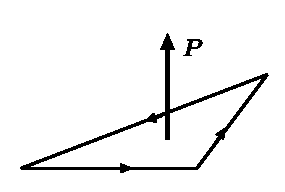
\includegraphics[scale=1.0]{pics/dipol.eps}}

S druge strane, veća D$_3$ simetrija ukida takvu mogućnost. $b$-rotacija
mijenja $\vec{P}\to-\vec{P}$ pa bi $\vec{P}\neq 0$ narušilo simetriju.

\centerline{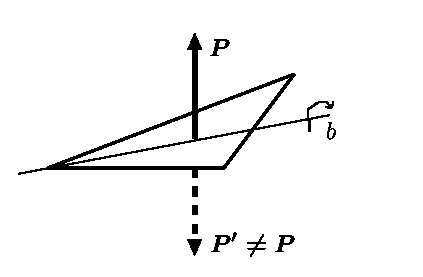
\includegraphics[scale=1.0]{pics/nodipol.eps}}

Atomi simetričnog kristala ne mogu proizvesti nesimetrični dipolni moment.

Grupno-teorijski iskaz ovoga je da \emph{reprezentacija grupe $G$ na vektorskom
prostoru (potencijalnih) vektora dipolnog momenta mora biti trivijalna tj.
identiteta}:
\begin{displaymath}
   D(g)=1 \quad \forall g\in G \;.
\end{displaymath}
Dakle, da bi kristal mogao imati $\vec{P}\neq 0$, reprezentacija grupe $G$ na 
3D euklidskom vektorskom prostoru mora 
u svojoj dekompoziciji na ireducibilne reprezentacije sadržavati identitetu,
a odgovarajući invarijantni potprostor je prostor mogućih vektora dipolnog momenta.

Vidjeli smo u prošlom odjeljku da se reprezentacija $\Gamma_V$ grupe D$_3$ na 3D
euklidskom vektorskom prostoru rastavlja na ireducibilne kao
\begin{displaymath}
             \Gamma_V = A_2 \oplus E \;,
\end{displaymath}
pa kako u tom rastavu nema trivijalne reprezentacije $A_1$, zaključujemo
da kristal sa D$_3$ simetrijom ne može imati električni dipolni moment.
S druge strane, uvjerite se da za C$_3$ vrijedi
\begin{displaymath}
             \Gamma_V = A_1 \oplus E \;,
\end{displaymath}
gdje je $A_1$ trivijalna reprezentacija
pa u ovom slučaju postoji mogućnost električnog dipolnog momenta.


Kad grupa simetrija pored rotacija sadrži i refleksije ($\sigma$, $S_n$, $i$,
vidi odjeljak \ref{sec:kristalografija}) treba
uzeti u obzir činjenicu da je magnetski moment $\vec{M}$ \emph{aksijalni}
vektor (vidi Dodatak \ref{sec:aksijalni})
koji se pri takvim transformacijama ponaša obrnuto od običnog
(polarnog) vektora električnog dipolnog momenta.
Tako npr. refleksija preko horizontalne ravnine $\sigma_h$ će promijeniti
predznak vertikalno usmjerenog električnog, ali ne i
magnetskog dipolnog dipolnog momenta:

\centerline{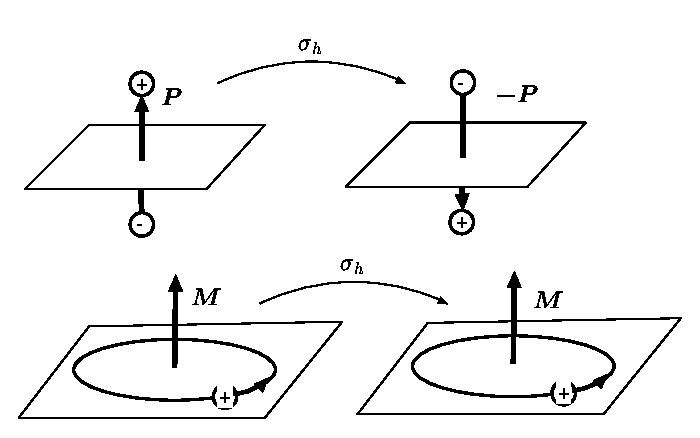
\includegraphics[scale=0.8]{pics/aksijal1.eps}}

Isto tako, refleksija preko vertikalne ravnine $\sigma_v$ neće promijeniti
predznak vertikalno usmjerenog električnog, ali hoće
magnetskog dipolnog dipolnog momenta\footnote{ 
Usput, razmislite zašto ogledalo izvrće lijevo-desno, a ne i gore-dolje? Promatrajući
operaciju refleksije preko vertikalnog ogledala koje leži
u $x-z$ ravnini $\sigma_v:(x, y, z)\mapsto (x, -y, z)$
čini se da bi ta dva smjera trebala biti ekvivalentna.}.

\centerline{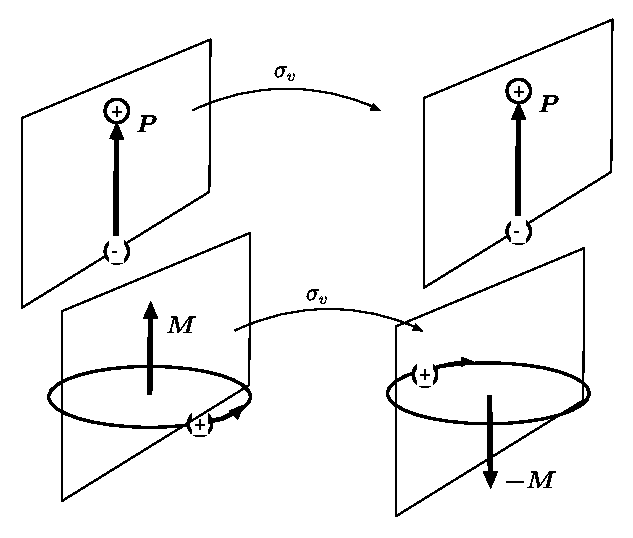
\includegraphics[scale=0.8]{pics/aksijal2.eps}}


Uzmimo kao primjer kristal s C$_{3v}$ simetrijom.
Grupa C$_{3v}$ je izomorfna grupi D$_3$, jedino što $b$ nije rotacija
za $\pi/2$ oko horizontalne osi već refleksija oko vertikalne ravnine
koja sadrži $C_3$ os\footnote{Vidimo da ovdje grupe ne razmatramo sasvim 
apstraktno nego koristimo različite oznake za jednu te istu apstraktnu
grupu imajući u vidu zapravo različite reprezentacije na euklidskom
vektorskom prostoru.}.

Reprezentacija elemenata $e, c$ i  $c^2$ je kao u primjeru \ref{pr:repC3},
\begin{displaymath}
D(c)=
\left(
\begin{array}{ccc}
-1/2 & -\sqrt{3}/2 & 0 \\
\sqrt{3}/2 & -1/2 & 0 \\
0 & 0 & 1
\end{array}\right) \;, \ldots
\end{displaymath}
s karakterima $\chi^{(V)}(e)=\mbox{dim}\Gamma_{V}=3$, $\chi^{(V)}(c)=0$,
a ako osi izberemo kao na slici

\centerline{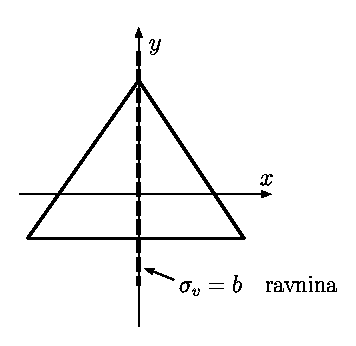
\includegraphics[scale=0.8]{pics/C3vravnina.eps}}

onda je 

\begin{displaymath}
D^{(V)}(b)=
\begin{pmatrix}
-1 & 0 & 0 \\
0 & 1 & 0 \\
0 & 0 & 1
\end{pmatrix}
\end{displaymath}
s karakterom $\chi^{(V)}(b)=1$ (usporedite s (\ref{eq:DVbD3})).
Kako je grupa C$_{3v}$ izomorfna grupi D$_3$ ima istu tablicu karaktera\footnote{Obrat
ne vrijedi, npr. Q i T$_d$ imaju iste tablice karaktera, a nisu izomorfne.}. Dakle,
imamo
\begin{center}
\begin{tabular}{c|ccc}
  & E & 2$C_3$  & 3$C_2$ \\ \hline
$A_1$ & 1 & 1& 1 \\
$A_2$ & 1 & 1&-1 \\
 $E$  & 2 &-1& 0 \\ \hline
 $\Gamma_V$ & 3 & 0 & 1
\end{tabular}
\end{center}

iz čega slijedi
\begin{displaymath}
   \Gamma_{V} = A_1  \oplus E \,.
\end{displaymath}
Kako se u rastavu javlja trivijalna reprezentacija $A_1$  slijedi
da je za ovaj kristal moguć permanentni \emph{električni} dipolni
moment.

Za aksijalne vektore, reprezentacije elemenata $e, c$ i $c^2$ su iste kao i
gore, jer rotacije ne razlikuju polarne i aksijalne vektore. 
Međutim refleksija $D^{(V)}(b)$ je reprezentirana
suprotno\footnote{Oblik matrice se može naći i iz razmatranja djelovanja $\sigma_{v}$ na
aksijalni vektor $\vec{c}=\vec{a}\times\vec{b}$ gdje 
su $\vec{a}$ i $\vec{b}$ pravi
vektori. Imamo $\sigma_{v}:(a_x, a_y, a_z)\mapsto (-a_x, a_y, a_z)$ i
 analogno $\sigma_{v}:(b_x, b_y, b_z)\mapsto (-b_x, b_y, b_z)$ pa je
 $\sigma_{v}:(c_x, c_y, c_z)\mapsto (c_x, -c_y, -c_z)$.} 
od $D^{(V)}(b)$
\begin{displaymath}
D^{(V)}(b)=
\begin{pmatrix}
1 & 0 & 0 \\
0 & -1 & 0 \\
0 & 0 & -1
\end{pmatrix}
\end{displaymath}
s karakterom $\chi^{(A)}(b)=-1$.

Dakle, ukupni karakter reprezentacije je $\chi^{(A)}=(3, 0, -1)$ odnosno
\begin{displaymath}
      \Gamma_{A} = A_2 \oplus E \,.
\end{displaymath}
Tu se ne pojavljuje trivijalna $A_1$ pa ne može biti ni permanentnog \emph{magnetskog}
dipolnog momenta.

\section{Primjena: \emph{Degeneracija i cijepanje energijskih nivoa}}
\label{sec:degeneracija}

U kvantnoj mehanici stanja sustava su reprezentirana vektorima
$|\alpha\rangle$ u Hilbertovom vektorskom prostoru. Transformacije
sustava realiziramo djelovanjem odgovarajućih operatora $U$ na tom prostoru
\begin{equation}
 |\alpha'\rangle = U |\alpha\rangle \,,
\end{equation}
ili, ekvivalentno, transformacijom sličnosti drugih 
operatora $A$ koji djeluju u tom prostoru:
\begin{equation}
   A' = U^{-1} A U \,.
\end{equation}
Malo opsežniju rekapitulaciju relevatnih osnova može se naći u dodatku
\ref{sec:qm}, gdje je i objašnjeno da su operatori transformacije $U$
redovito unitarni. To sve vrijedi bez obzira na to je li transformacija
simetrija ili nije.

Kvantnomehanički sustav, zadan
hamiltonijanom $H_0$, je \emph{simetričan} obzirom na skup transformacija
$\{ U(g_1), U(g_2), \ldots, U(g_n)\}$ ako transformacije ne mijenjaju
hamiltonijan. 
\begin{equation}
    H_{0}' = U^{-1}(g) H_{0} U(g) = H_{0} \quad \forall  g \in \{g_1,\ldots, g_n\}\;.
 \label{eq:invH0}
\end{equation}
Naime, možemo reći da putem Schr\"{o}dingerove jednadžbe 
hamiltonijan definira sustav. Transformirani sustav će u slučaju da
je transformacija simetrija imati isti skup rješenja Schr\"{o}dingerove jednadžbe,
s istim energijama.
Ekvivalentno, iz (\ref{eq:invH0}) se vidi da tada operator
simetrije $U(g)$ i hamiltonijan $H_0$ komutiraju
\begin{equation}
  H_{0}U(g)=U(g)H_0 \quad \forall  g \in \{g_1,\ldots, g_n\} \;.
  \label{eq:comHU}
\end{equation}
Skup svih operatora s ovim svojstvom čini grupu (provjerite da su
zadovoljeni svi aksiomi grupe!) tj.
reprezentaciju grupe $G=\{g_1,\ldots, g_n\}$ na prostoru kvantnomehaničkih 
stanja.

Stanje sustava $|n\rangle$ s dobro definiranom energijom  zove se
\emph{stacionarno stanje} i dano je kao rješenje vremenski 
neovisne Schr\"{o}dingerove jednadžbe tj. kao svojstveno stanje hamiltonijana
\begin{displaymath}
  H_0 |n\rangle = E_n | n \rangle \;.
\end{displaymath}
Energija transformiranih stanja $|n'\rangle = U(g)|n\rangle$ je
odgovarajuća svojstvena vrijednost hamiltonijana pa zahvaljujući
(\ref{eq:comHU}) imamo
\begin{displaymath}
  H_0 |n'\rangle = H_0 U(g)|n\rangle = U(g) H_0 |n\rangle =
 U(g) E_n |n\rangle = E_n |n'\rangle \;.
\end{displaymath}
Dakle sva stanja $|n'\rangle = U(g)|n\rangle$, za sve $g\in G$ imaju
istu energiju $E_n$! Pojavu kad više stanja ima istu energiju 
nazivamo \emph{degeneracija}.

Skup stanja $\{U(g)|n \rangle \,|\, g\in G\}$ dobivenih transformacijama
datog stanja $|n\rangle$ razapinje
potprostor vektorskog prostora svih stanja sustava. On je
po konstrukciji invarijantan na djelovanje reprezentacije $\{ U(g) \}$.
Također, reprezentacija $\{ U'(g) \}$ dobivena redukcijom reprezentacije
$\{ U(g) \}$ na ovaj potprostor je ireducibilna što isto slijedi
iz načina na koji smo konstruirali potprostor\footnote{Čitaoc će jako
profitirati ako pažljivo razmisli o ove dvije tvrdnje i detaljno se
uvjeri u njih tako da se uvjeri da djelovanjem operatora $\{ U(g) \}$
na vektore baze potprostora $\{U(g)|n \rangle \}$ nije moguće
dobiti vektor izvan tog potprostora (invarijantnost) te također da
je transformacijama bilo kojeg vektora baze moguće dobiti baš sve
ostale (ireducibilnost)}.
Takav potprostor naziva se \emph{multiplet}, a u literaturi se
vrlo često izraz multiplet koristi i za samu bazu ovog potprostora.

Vidimo da poznavajući sve ireducibilne reprezentacije grupe simetrija nekog
kvantnomehaničkog
sustava možemo odrediti mogućnosti degeneracije njegovih stanja.
One su upravo jednake dimenzionalnostima ireducibilnih reprezentacija.
Obrnuto, ako u prirodi uočimo degeneraciju, od koristi je identificirati
simetriju koja tu degeneraciju uzrokuje. Jednakost energija, dakle jednakost
realnih brojeva, teško može biti slučajna. Kad tako odredimo simetrije,
to nam može pomoći u određivanju strukture sustava i interakcija koje
njime upravljaju jer sve to mora biti u skladu sa simetrijama.

\begin{primjer}[Sustav s oktahedralnom grupom simetrija]

Ireducibilne reprezentacije oktahedralne grupe O pronađemo
u dodatku {sec:tablice} gdje vidimo 
da ta grupa ima dvije jednodimenzionalne
ireducibilne reprezentacije $A_1$ i $A_2$, jednu
dvodimenzionalnu $E$ i dvije trodimenzionalne $T_1$ i  $T_2$.
Očekujemo dakle da sustav ima jedno-, dvo- i trostruko degenerirane
energijske nivoe.
Recimo, energijski spektar i pripadajuće valne funkcije sustava mogle
bi biti organizirane ovako:

\hspace*{2cm}
\rule{3cm}{1pt}\hspace*{-3cm}%
\rule[2pt]{3cm}{1pt}\hspace*{-3cm}%
\rule[4pt]{3cm}{1pt}\hspace{12pt}%
$\psi_{T_1,1}, \psi_{T_1,2}, \psi_{T_1,3}$

\hspace*{2cm}
\rule{3cm}{1pt}\hspace*{12pt}%
$\psi_{A_2}'$

\hspace*{2cm}
\rule{3cm}{1pt}\hspace*{12pt}%
$\psi_{A_1}$

\hspace*{2cm}
\rule{3cm}{1pt}\hspace*{-3cm}%
\rule[2pt]{3cm}{1pt}\hspace*{12pt}%
$\psi_{E,1}, \psi_{E,2}$

\hspace*{2cm}
\rule{3cm}{1pt}\hspace*{12pt}%
$\psi_{A_2}$

Ovdje su $\psi_{A_2}'$ i $\psi_{A_2}$ linearno neovisne funkcije.
Pronađemo li ipak mjerenjima neki nivo s prevelikom degeneracijom,
npr.

\hspace*{2cm}
\rule{3cm}{1pt}\hspace*{-3cm}%
\rule[2pt]{3cm}{1pt}\hspace*{-3cm}%
\rule[4pt]{3cm}{1pt}\hspace{12pt}%
$\psi_{E,1}, \psi_{E,2}, \psi_{A_1}$

to gotovo uvijek znači da nismo dobro identificirali grupu simetrija
tj. da sustav ima veću simetriju nego što smo mislili. U ovom slučaju
vjerojatno postoji transformacija čiji operator komutira s hamiltonijanom i
koji povezuje degenerirana stanja, npr.
\begin{displaymath}
 U(h) \psi_{E,1} = \psi_{A_1} \,,
\end{displaymath}
gdje $h$ nije element oktahedralne grupe O nego tek treba otkriti veću grupu kojoj
on pripada i kojoj je O podgrupa.

\end{primjer}


\begin{primjer}[Sferna simetrija i vodikov atom]


Ukoliko zanemarimo interakcije višeg reda (poput interakcije spina i orbite) i
promatramo samo osnovni hamiltonijan vodikovog atoma po kojem se elektron nalazi u kulonskom 
električnom polju jezgre u ishodištu, vidimo da sustav ima sfernu simetriju --- simetriju
na sve rotacije 3D prostora oko ishodišta. Odgovarajuća grupa simetrija je
beskonačnog reda i zove se SO(3).
U poglavlju \ref{ch:rotacije} ćemo naučiti da su multipleti te SO(3)
simetrije $(2l+1)$-dimenzionalni.
Stoga očekujemo $(2l+1)$-struko degenerirane nivoe za svaki $l$. 
Važno je razumjeti da je to općenita algebarska posljedica sferne simetrije.
Svaki sferno-simetrični sustav, bez obzira na njegov konkretni sastav
i hamiltonijan, imat će prirodno pridruženi kvantni broj $l$
i odgovarajuće $(2l+1)$-struko degenerirane energijske nivoe u svojem spektru.

I zaista, rješavanjem Schr\"{o}dingerove jednadžbe za vodikov atom
dobivamo rješenja koja labeliramo
s trima kvantnim brojevima  $\psi_{nlm}(\vec{x}) = \langle \vec{x} | nlm \rangle$. 
i stanja
\begin{displaymath}
   \{ \psi_{nl(-l)}, \psi_{nl(-l+1)}, \ldots, \psi_{nll}\} \;,
\end{displaymath}
zaista jesu degenerirana.
No dodatno cijela ljuska s konkretnom vrijednošću kvantnog broja $n$, a
koja sadrži $n^2$ stanja s $l \in \{0, 1, \ldots, n-1\}$
ima istu energiju
\begin{displaymath}
  E_n \propto \frac{1}{n^2} \qquad \text{neovisno o $l$}
\end{displaymath}
Dakle, degeneracija je veća od one koju bismo očekivali samo zbog
sferne simetrije SO(3).
U odjeljku \ref{sec:so4}  ćemo vidjeti da je relevantna simetrija
zapravo SO(4)=SO(3)$\otimes$SO(3) što će onda kompletno objasniti
opaženu degeneraciju nivoa vodikovog atoma.
\end{primjer}

Tako teorija grupa omogućuje neke spoznaje o spektru sustava
čak i ako ne znamo riješiti njegovu Schr\"{o}dingerovu jednadžbu.
No i onda kada znamo riješiti Schro\"{o}dingerovu
jednadžbu sustava, teorija grupa nam može biti od pomoći
da bolje razumijemo rješenje ili da si uštedimo dio posla jer
na primjer ako znamo da su neki nivoi degenerirani, dovoljno je izračunati
energiju samo jednog od njih.

\subsection*{Cijepanje energijskih nivoa}

Vidjeli smo kako struktura grupe simetrija sustava diktira moguće
ireducibilne reprezentacije, a one pak diktiraju mogućnost 
degeneracija u energijskom spektru sustava. Zanimljivo je promotriti
što se događa sa spektrom ukoliko se simetrija sustava promijeni.
Razlog promjeni može biti na primjer promjena kristalne strukture
zbog promjene temperature ili promjena simetrije zbog uključivanja
vanjskog električnog ili magnetskog polja.
Konkretno, zamislimo da uvođenje vanjskog potencijala $V$  promijeni hamiltonijan
sustava
\begin{displaymath}
    H_0 \to H = H_0 + V \;.
\end{displaymath}
Ukoliko znamo riješiti sustav opisan osnovnim hamiltonijanom $H_0$, te
ukoliko je smetnja $V$ slaba ($V\ll H_0$), tehnikama računa smetnje
moguće je  odrediti promjene energijskih nivoa. No, ukoliko je takav
pristup težak ili nemoguć, već i tehnike teorije grupa mogu dati neki uvid
u promjene u spektru sustava. 

Pretpostavimo da je originalni hamiltonijan $H_0$ invarijantan na
grupu simetrija $G$. Uvođenje smetnje $V$ će u najvećem broju
slučajeva smanjiti simetriju tako da će ukupni hamiltonijan $H$ 
biti sada invarijantan na manju grupu $H<G$. To je jasno jer 
hamiltonijan $H_0$ komutira sa svim operatorima koji reprezentiraju
grupu simetrija $G$. Ako hamiltonijanu dodamo novi član $V$, neki operatori iz
tog skupa $\{U(g) \td g\in G\}$ tipično neće komutirati i s $H_0 + V$.
Na primjer, električno polje u Starkovom efektu mijenja Hamiltonijan
vodikovog atoma tako da mu doda član proprocionalan električnom polju
i od originalne pune sferne simetrije na sve rotacije 3D prostora,
preostaje samo aksijalna simetrija na rotacije oko smjera polja.

Ireducibilne reprezentacije grupe $G$ nisu nužno i ireducibilne
reprezentacije grupe $H$. Smanjenje broja transformacija
$U(h)$, $h\in H$ može učiniti da neki potprostori postanu invarijantni
iako nisu bili invarijantni na potpun skup transformacija $U(g)$, $g\in G$.
Tako su neke ireducibilne reprezentacije od $G$ reducibilne obzirom na $H$
i nema razloga da energijski nivoi koji odgovaraju dotičnim reprezentacijama
od $G$ ostanu degenerirani nakon uvođenja smetnje.

\centerline{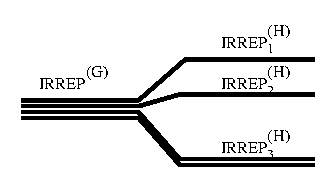
\includegraphics[scale=1.0]{pics/splitting.eps}}
 
Poznavajući dekompoziciju ireducibilne reprezentacije $IRREP^{(G)}$
grupe $G$ na ireducibilne reprezentacije  $IRREP^{(H)}$ grupe $H$
\begin{displaymath}
   IRREP^{(G)}=(\text{reducibilna REP})^{(H)}=
 IRREP^{(H)}_1 \oplus IRREP^{(H)}_2 \oplus \cdots
\end{displaymath}
možemo odrediti strukturu cijepanja. Za određivanje \emph{iznosa} cijepanja
trebat će tipično ipak koristiti metode kvantnomehaničkog računa smetnje.

\begin{primjer}[Cijepanje $T$-nivoa tetrahedralne grupe T]

Ireducibilna reprezentacija $T$, tetrahedralne grupe T, je
trodimenzionalna, pa će odgovarajući nivo biti trostruko degeneriran
(tri različita kvantna stanja će imati istu energiju).
Karakter $T$-nivoa tetrahedralne grupe je
\begin{displaymath}
\begin{tabular}{c|cccc}
  & E & 3$C_2$  & 4$C_3$ & 4$C_{3}'$ \\ \hline
 $T$ & 3  & -1 & 0 & 0 
\end{tabular}
\end{displaymath}

Zamislimo da sada kristal s tetrahedranom grupom simetrija doživi
fazni prijelaz tako da se
simetrija smanji a) $\mathrm{T}\to \mathrm{D}_2$ ili b) $\mathrm{T}\to
\mathrm{C}_{3v}$. Pogledajmo
što se događa s gornjim trostruko degeneriranim nivoom.

a) $\mathrm{T}\to \mathrm{D}_2$. Uspoređujući strukture dvaju grupa,
vidimo da transformacije iz klasa $C_3$ i $C_{3}'$ više nisu simetrije
jer u grupi $\mathrm{D}_2$ uopće nema transformacija $C_3$ tipa koje
su reda 3. Isto tako, tri transformacije iz klase $C_2$ su i dalje
simetrije, ali više nisu u jednoj klasi konjugacije nego su sve tri
u zasebnim klasama. Tako vidimo da karakteri $T$-nivoa odgovaraju
karakterima grupe D$_2$ kako je prikazano na sljedećoj tablici

\begin{displaymath}
\begin{tabular}{c|cccc}
 & $E$  & $C_{2}^z$ &  $C_{2}^y$ & $C_{2}^x$ \\ \hline
$A_1$ & 1 & 1& 1 & 1 \\
$B_1$ & 1 & 1&-1  & -1\\
$B_2$ & 1 & -1&1  & -1\\
$B_3$ & 1 & -1&-1  & 1\\ \hline \hline
 $T$ & 3 & -1 & -1 & -1
\end{tabular}
\end{displaymath}

Sada provodimo dekompoziciju reprezentacije $T$ koja je u kontekstu
grupe D$_2$ reduciblilna
\begin{displaymath}
   T = a_1 A_1 \oplus b_1 B_1 \oplus b_2 B_2 \oplus b_3 B_3
\end{displaymath}
Mulitiplicitete određujemo skalarnim množenjem redaka gornje tablice:
\begin{align*}
a_1 &= \frac{1}{n}\sum_k \chi^{(A_1)}(k) \chi^{(T)^*}(k)  \\
    &= \frac{1}{4}\big(1\cdot3 + 1\cdot(-1) + 1\cdot(-1) + 1\cdot(-1)\big) = 0 \\
b_1 &= b_2 = b_3 = 1
\end{align*}
Dakle degeneracija je potpuno ukinuta
\begin{displaymath}
  \imp   T =  B_1 \oplus B_2 \oplus B_3
\end{displaymath}

\centerline{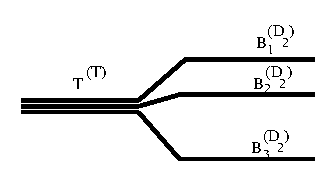
\includegraphics[scale=1.0]{pics/splittingT.eps}}

b) $\mathrm{T}\to \mathrm{C}_{3v}$. Sličnim postupkom dobivamo
\begin{displaymath}
        T = A_2 \oplus E \;,
\end{displaymath}
tj. degeneracija je samo djelomično ukinuta

\centerline{\includegraphics[scale=1.0]{pics/splittingT2.eps}}

\end{primjer}

\subsection*{Zadaci}

\begin{enumerate}[label=\arabic{chapter}.\arabic*.]

\item Konstruirajte 2D IRREP grupe $D_3$ koja djeluje na $x-y$ ravnini
i provjerite temeljni teorem o ortogonalnosti.

\item Pokažite da su sve IRREP Abelovih grupa jednodimenzionalne.
    \label{zad:1Dabelrep}

\item Pokažite da je nužan i dovoljan uvjet ireducibilnosti reprezentacije
 $\Gamma$ s karakterima $\chi_i$ tzv. Frobeniusov kriterij
\begin{displaymath}
    \sum_i k_i |\chi_i|^2 = n  \;,
\end{displaymath}
gdje je $k_i$ broj elemenata u klasi konjugacije $i$.

\item Konstruirajte tablicu karaktera za grupu $D_4$

\item Pokažite da je direktni produkt dvije 1D IRREP uvijek IRREP.

\item Izrazite reprezentaciju $\Gamma$ grupe $C_{4v}$ koja ima
karaktere
\begin{displaymath}
  \chi(E)=5\;,\; \chi(C_2)=1\;,\; \chi(C_4)=-1\;,\;
  \chi(\sigma_v)=1\;,\; \chi(\sigma_d)=-3\;,
\end{displaymath}
kao zbroj IRREPsa.
\end{enumerate}
